%%%%%%%%%%%%%%%%%%%%%%%%%%%%%%%%%%%%%%%%%
% Beamer Presentation
% LaTeX Template
% Version 1.0 (10/11/12)
%
% This template has been downloaded from:
% http://www.LaTeXTemplates.com
%
% License:
% CC BY-NC-SA 3.0 (http://creativecommons.org/licenses/by-nc-sa/3.0/)
%
%%%%%%%%%%%%%%%%%%%%%%%%%%%%%%%%%%%%%%%%%

%----------------------------------------------------------------------------------------
%	PACKAGES AND THEMES
%----------------------------------------------------------------------------------------

\documentclass{beamer}

\mode<presentation> {

\usetheme{Madrid}

}

\definecolor{DataBlue}{rgb}{0.50, 0.85, 0.99} 
\definecolor{miptcolour}{rgb}{0.0, 0.45, 0.81}

\setbeamercolor{titlelike}{parent=structure,bg=miptcolour, fg = white}
\setbeamercolor{frametitle}{fg=white}
\usepackage{graphicx} % Allows including images
\usepackage{booktabs} % Allows the use of \toprule, \midrule and \bottomrule in tables
\usepackage[export]{adjustbox}
\usepackage{hyperref}
 \hypersetup{
     colorlinks=true,
     linkcolor=miptcolour,
     filecolor=miptcolour,
     citecolor=miptcolour,      
     urlcolor=miptcolour,
     }
\usepackage[backend=biber, sorting=none]{biblatex}

\addbibresource{references.bib}

%----------------------------------------------------------------------------------------
%	TITLE PAGE
%----------------------------------------------------------------------------------------

\title{L[0]: Representation of Chemical Compounds} %% Title
\author{Khalimat A. Murtazalieva} % Your name
\institute[MIPT] % Your institution as it will appear on the bottom of every slide, may be shorthand to save space
{
Fundamentals of Cheminformatics \\ % Your institution for the title page
\medskip
\textit{@khalimat} % Your email address
}
\date{\today} % Date, can be changed to a custom date

% Rodapé
\setbeamertemplate{footline}{%
    \begin{beamercolorbox}[wd=\paperwidth]{footlinecolor}
        
\includegraphics[width=\paperwidth]{images/footbar.png}
    \end{beamercolorbox}%
}

\begin{document}
{
\setbeamertemplate{footline}{} 
\begin{frame}
\begin{columns}
    \begin{column}{0.90\textwidth}
        \titlepage
    \end{column}
\end{columns}


\begin{figure}[b]
\center{
\includegraphics[width=0.1\linewidth]{images/hv_s_no_bg.png}}
\end{figure}

\end{frame}
}

\begin{frame}
\frametitle{Overview} % Table of contents slide, comment this block out to remove it
\tableofcontents % Throughout your presentation, if you choose to use \section{} and \subsection{} commands, these will automatically be printed on this slide as an overview of your presentation
\end{frame}

%----------------------------------------------------------------------------------------
%	PRESENTATION SLIDES
%----------------------------------------------------------------------------------------

%------------------------------------------------
\section{Line Notations} % Sections can be created in order to organize your presentation into discrete blocks, all sections and subsections are automatically printed in the table of contents as an overview of the talk
%------------------------------------------------

\begin{frame}
\frametitle{Line notations}
\begin{block}{Definition}
Line notations represent the structure of chemical compounds as a linear sequence
of letters and numbers. The \href{https://iupac.org/what-we-do/nomenclature/}{IUPAC nomenclature} represents such a kind of line
notation. There is a table below from \cite{gasteiger2006chemoinformatics} with examples of line notations.
\end{block}
\begin{figure}[h!]
\center{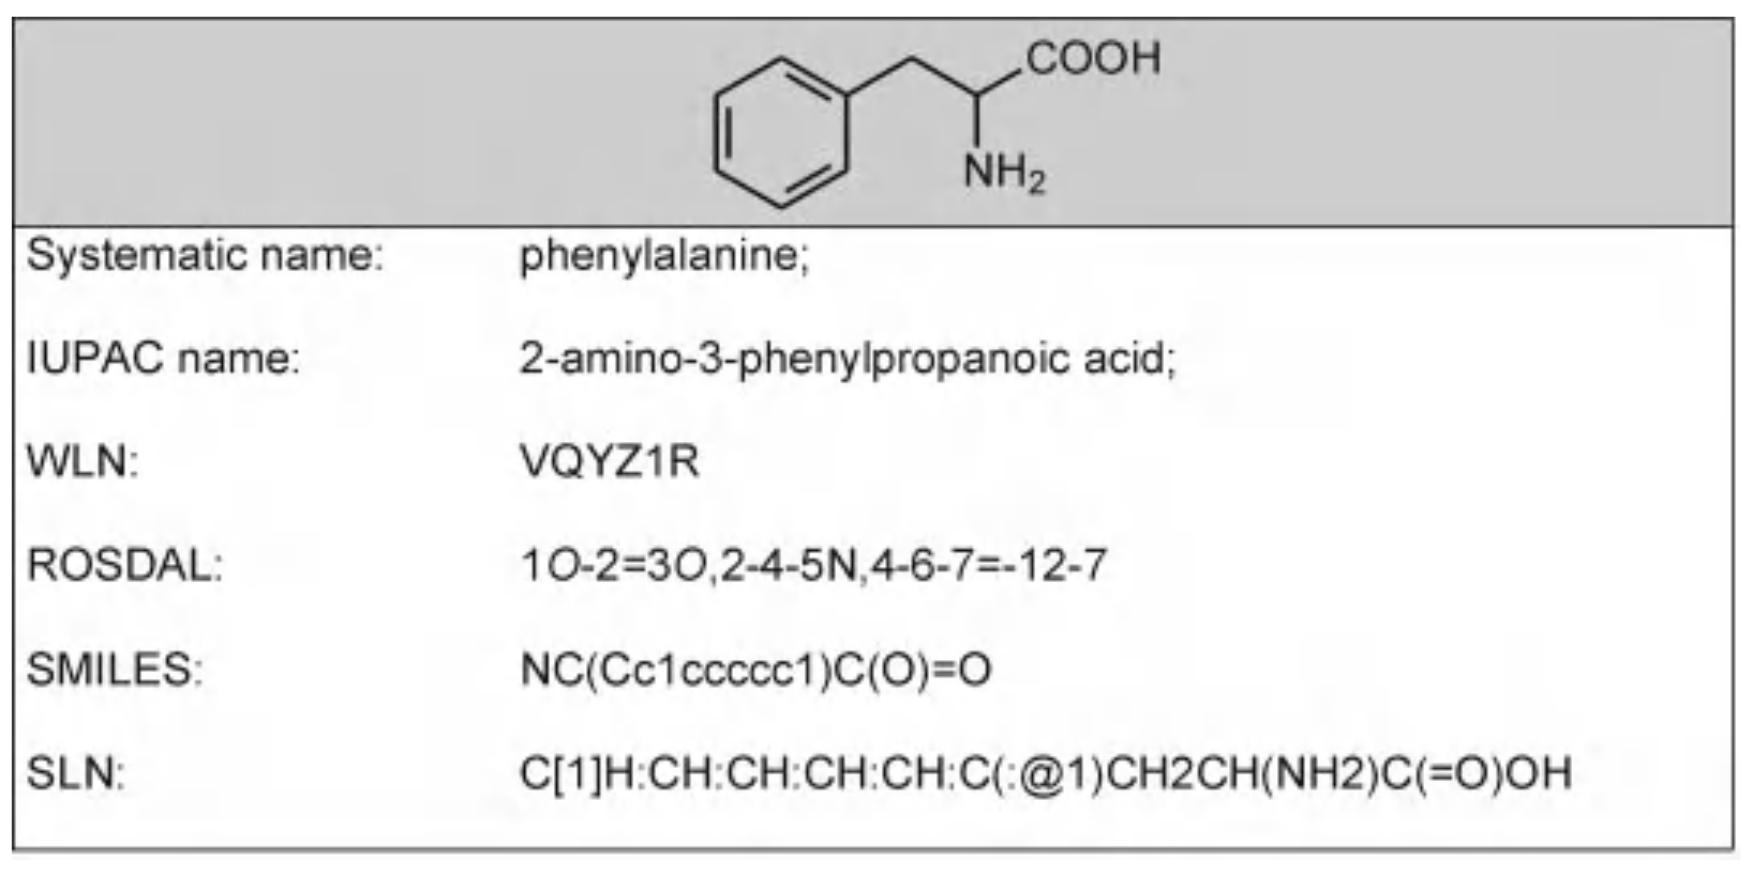
\includegraphics[width=0.55\linewidth]{images/Line_notations.png}}
\caption{Different line notations for the structure diagram of phenylalanine\cite{gasteiger2006chemoinformatics}.}
\end{figure}
\end{frame}

\subsection{SMILES} 
\begin{frame}
\frametitle{SMILES}
The SMILES (Simplified Molecular Input Line Entry System) Coding was developed by David Weininger in 1986 for chemical data processing. The advantages of this system are that it enables to compress and simplify chemical information. 
The basic SMILES rules are:
\begin{itemize}
\item Atoms are represented by their atomic symbols.
\item Hydrogen atoms automatically saturate free valences and are omitted (simple
hydrogen connection).
\item Neighboring atoms stand next to each other.
\item Double and triple bonds are characterized by  = and \#, respectively.
\item Branches are represented by parentheses.
\item Rings are described by allocating digits to the two "connecting" ring atoms.
\end{itemize}
Further information can be found \href{http://www.daylight.com/dayhtml/smiles/index.html}{here}.
\end{frame}


\begin{frame}
\frametitle{SMILES syntax, 1}

\begin{figure}[h!]
\center{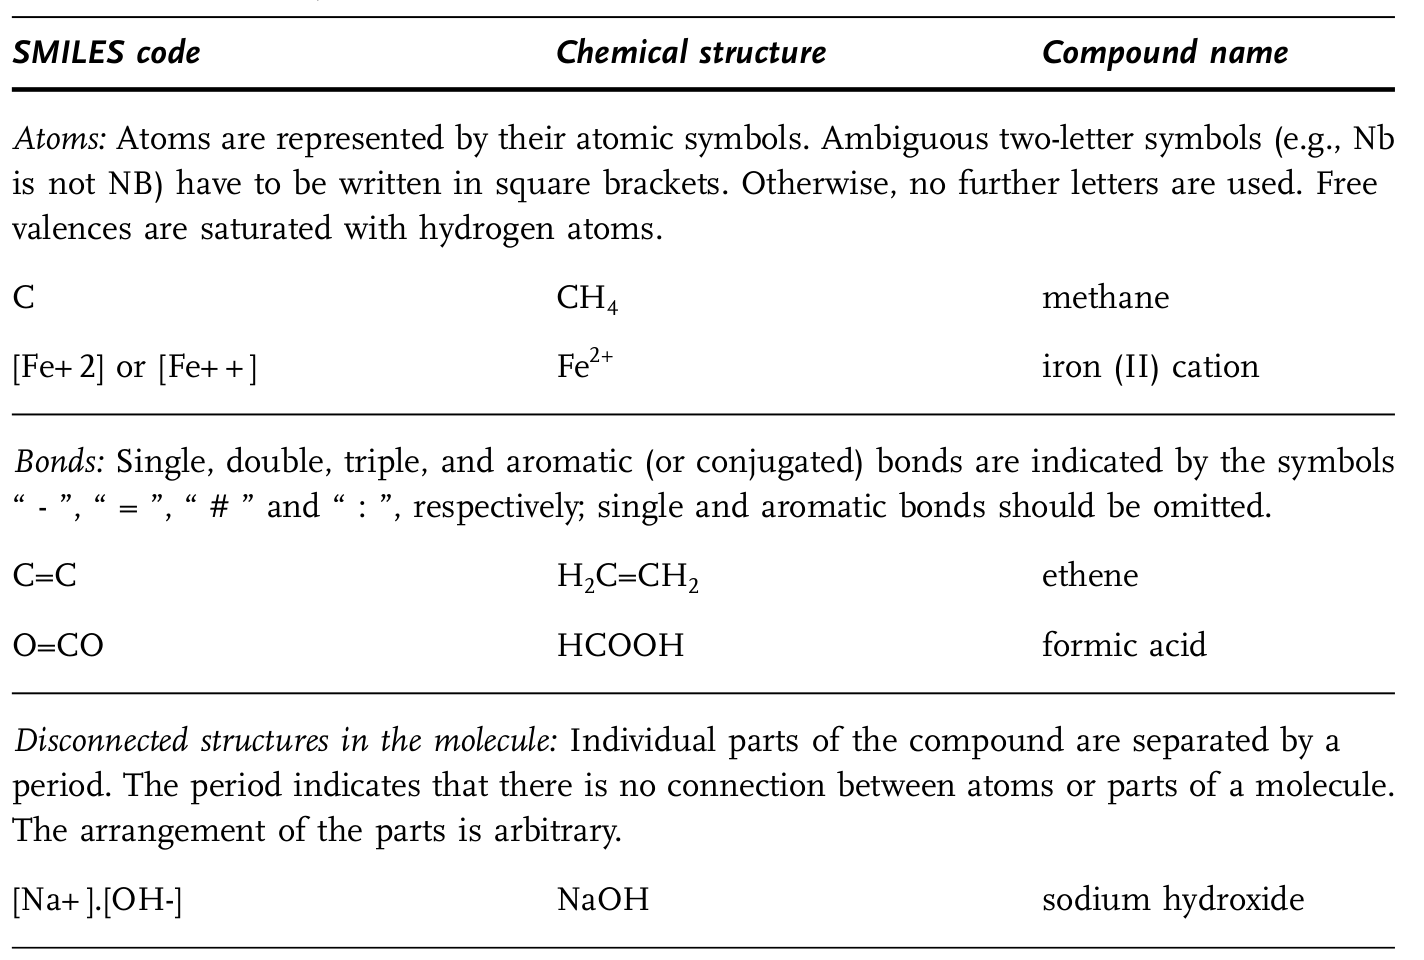
\includegraphics[width=0.83\linewidth]{images/SMILES_1.png}}
\caption{SMILES syntax, from \cite{gasteiger2006chemoinformatics}.}
\end{figure}
\end{frame}

\begin{frame}
\frametitle{SMILES syntax, 2}
\begin{figure}[h!]
\center{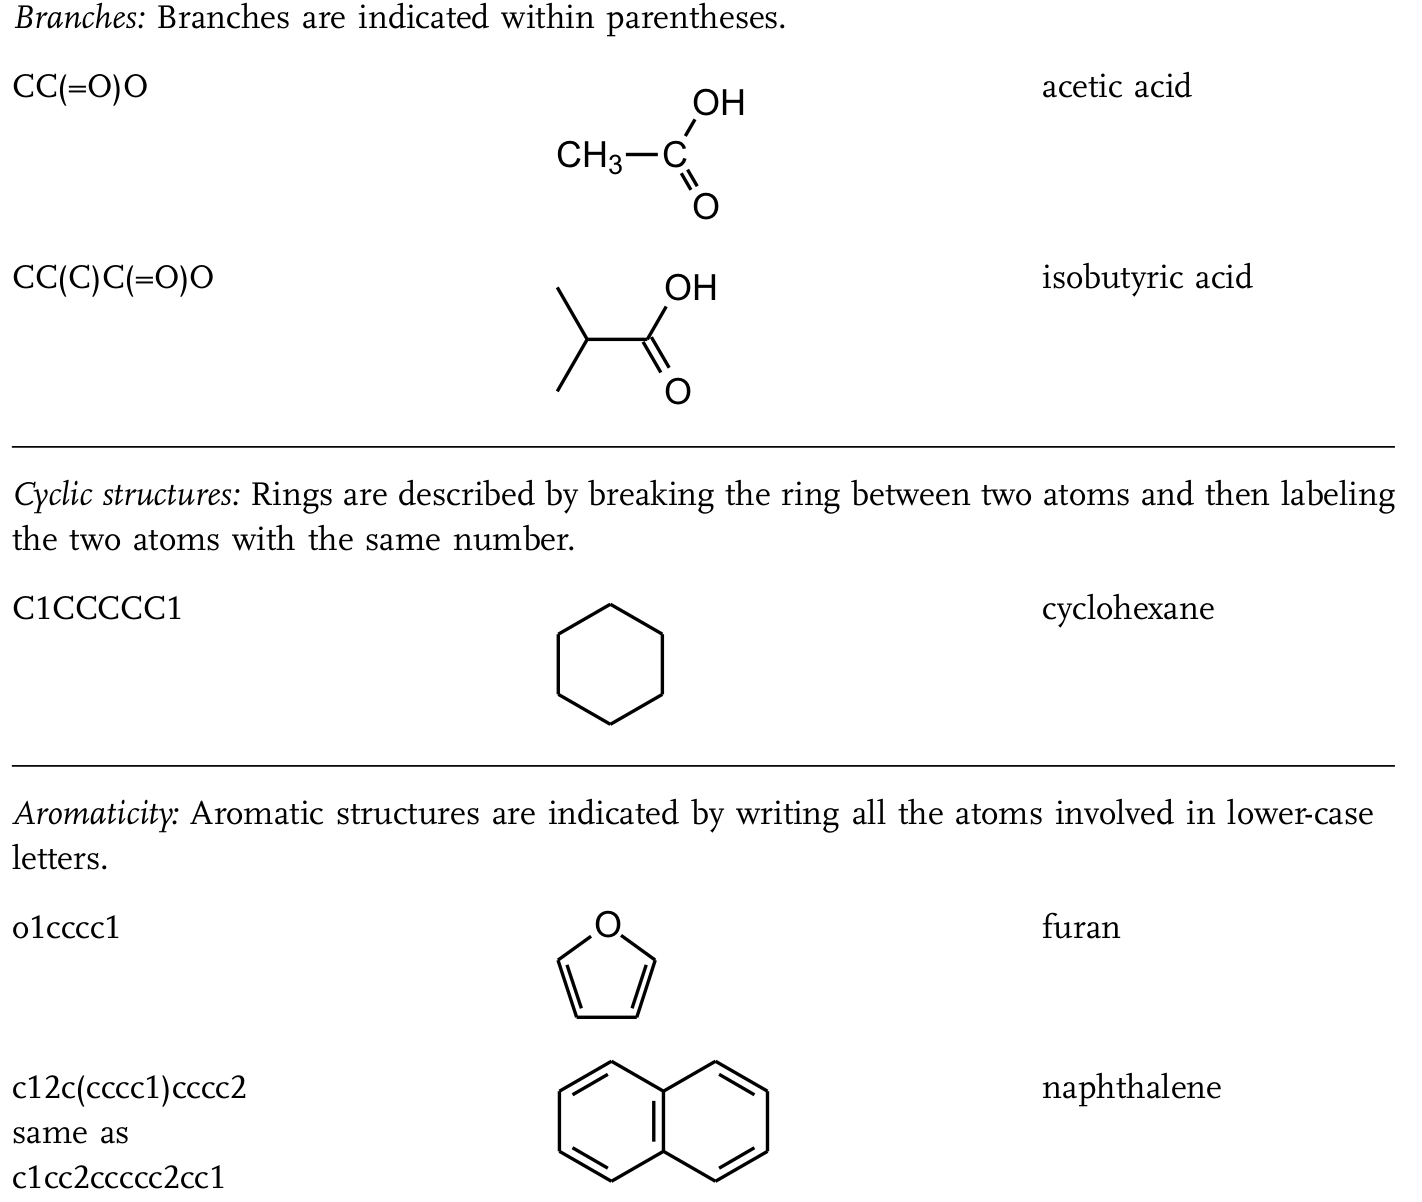
\includegraphics[width=0.73\linewidth]{images/SMILES_2.png}}
\caption{SMILES syntax, from \cite{gasteiger2006chemoinformatics}.}
\end{figure}
\end{frame}

\section{2D Notations} % Sections can be created in order to organize your presentation into discrete blocks, all sections and subsections are automatically printed in the table of contents as an overview of the talk
\subsection{Graph Notations}
\begin{frame}
\frametitle{Intro}
The analogy of structural diagrams to graphs is the reason why graph notations are widely used in cheminformatics. Hence, as a first step, we have to get acquainted with some basic definitions of graph theory. If you wish to achieve a deeper understanding, please pass \href{https://www.coursera.org/learn/teoriya-grafov}{this course}. For our course, please memorize everything from this short \href{https://stanford.edu/~rezab/classes/cme305/W14/Notes/2.pdf}{intro}.
Moreover, please read this \href{https://towardsdatascience.com/graph-data-structure-cheat-sheet-for-coding-interviews-a38aadf8aa87}{article}. You must be able to reproduce and apply algorithms from the article during our course. 
\begin{figure}[h!]
\center{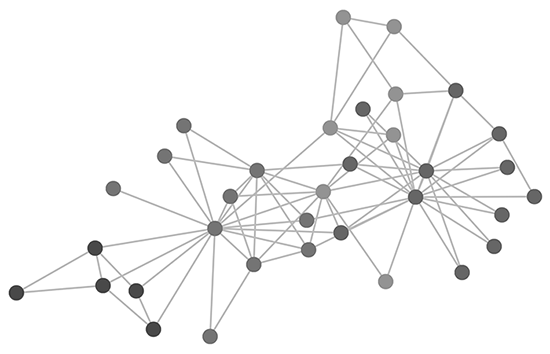
\includegraphics[width=0.4\linewidth]{images/Black-n-White.png}}
\caption{A graph}
\end{figure}
\end{frame}

\subsubsection{Matrix Representations}
\begin{frame}
\frametitle{Matrix Representations}
A graph can be represented as a matrix. Thus, quite early on, matrix representations of molecular structures were explored. Their major advantage is that the calculation of paths and cycles can be performed easily by well-known matrix operations. 
\begin{figure}[h!]
\center{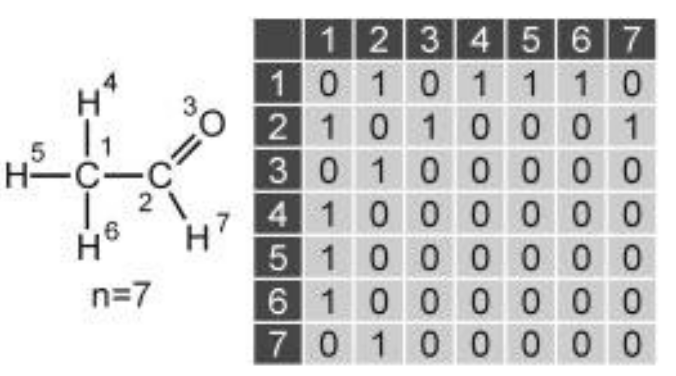
\includegraphics[width=0.4\linewidth]{images/ethanal.png}}
\caption{Adjacency matrix of ethanal\cite{gasteiger2006chemoinformatics}.}
\end{figure}
\end{frame}

\begin{frame}
\frametitle{Storage efficiency}
The matrix representation is redundant. Hence, it could be simplified by omitting the zero 0, reducing to the top triangle, and omitting the hydrogen atoms.       
 
\begin{figure}[h!]
\center{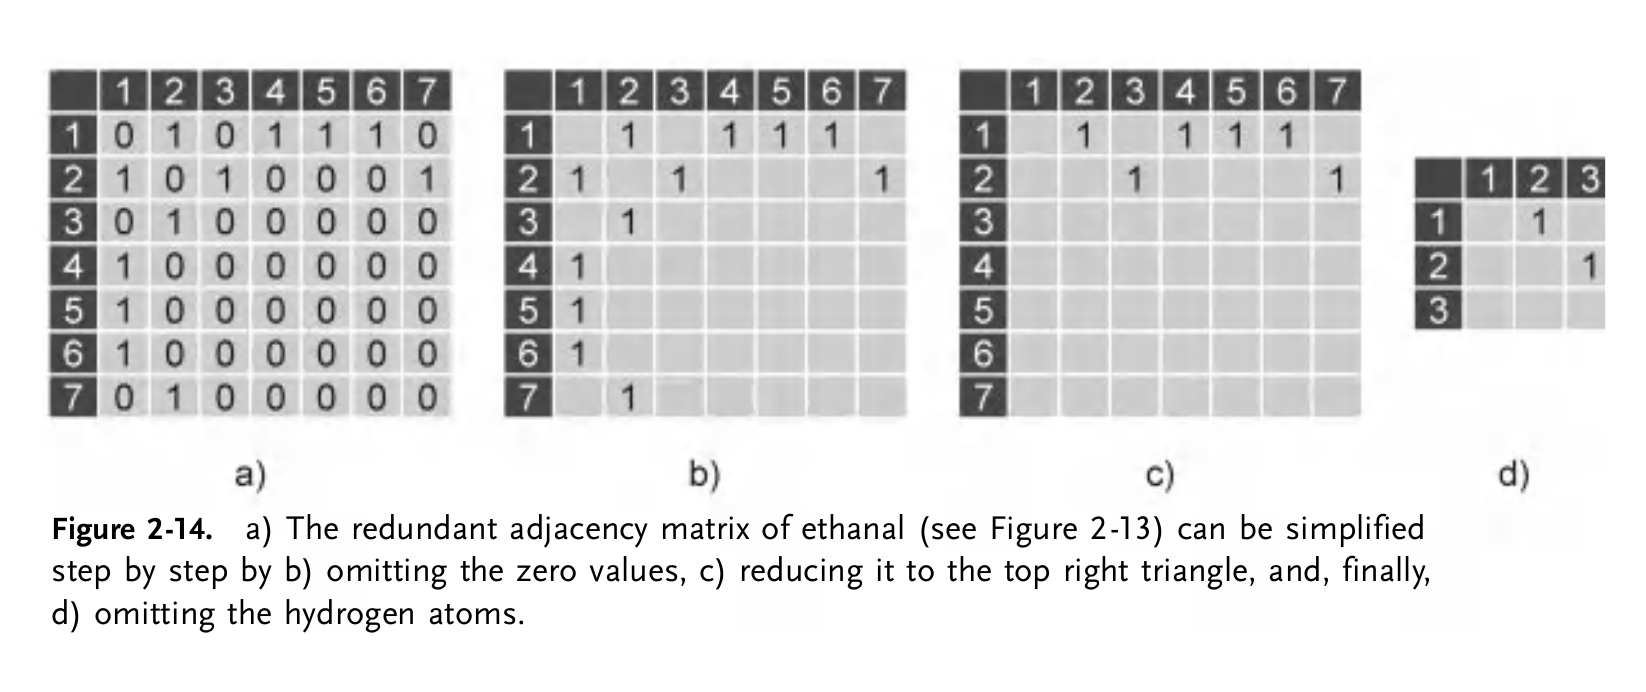
\includegraphics[width=0.88\linewidth]{images/simplify.png}}
\caption{A simplification procedure \cite{gasteiger2006chemoinformatics}.}
\end{figure}
\end{frame}
\subsubsection{Connection Table}
\begin{frame}
\frametitle{Connection Table}
A major disadvantage of a matrix representation for a molecular graph is that the number of entries increases with the square of the number of atoms in the molecule. What is needed is a representation of a molecular graph where the number of
entries increases only as a linear function of the number of atoms in the molecule. Such a representation can be obtained by listing, in tabular form only the atoms and the bonds of a molecular structure.      
 
\begin{figure}[h!]
\center{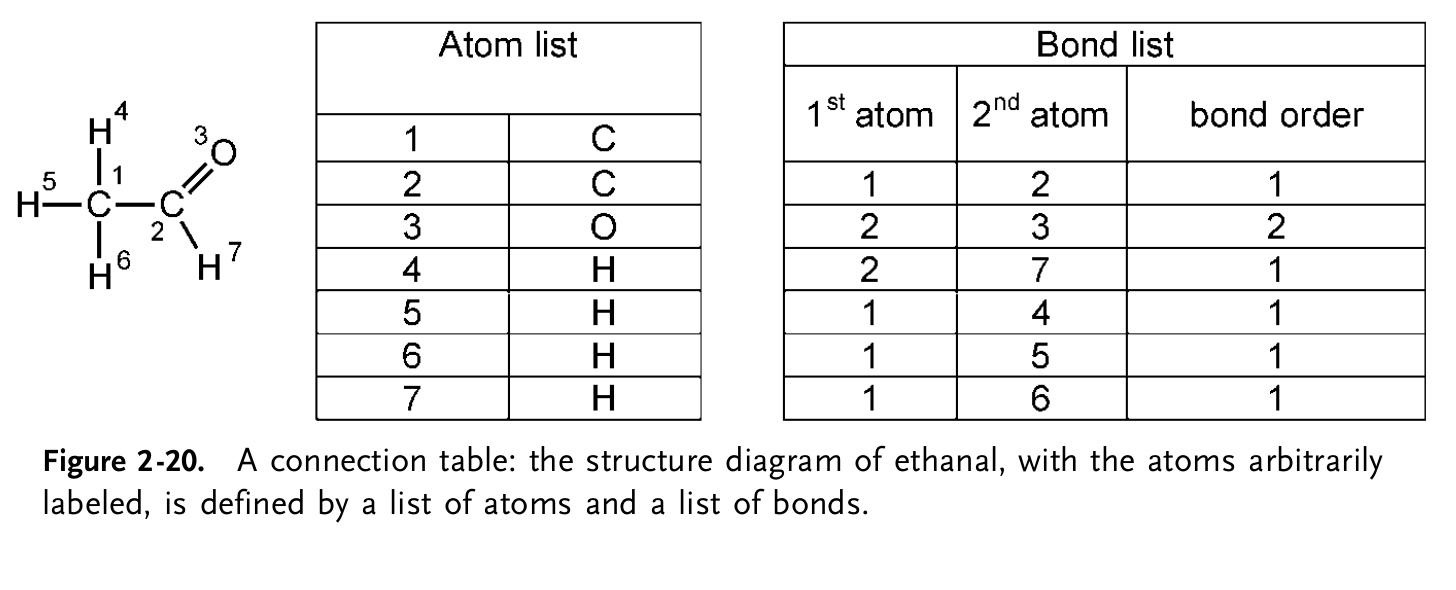
\includegraphics[width=0.80\linewidth]{images/connection_table.png}}
\caption{A simplification procedure \cite{gasteiger2006chemoinformatics}.}
\end{figure}
\end{frame}


\subsection{Standard Structure Exchange Formats}
\begin{frame}
\frametitle{Overview}

\begin{figure}[h!]
\center{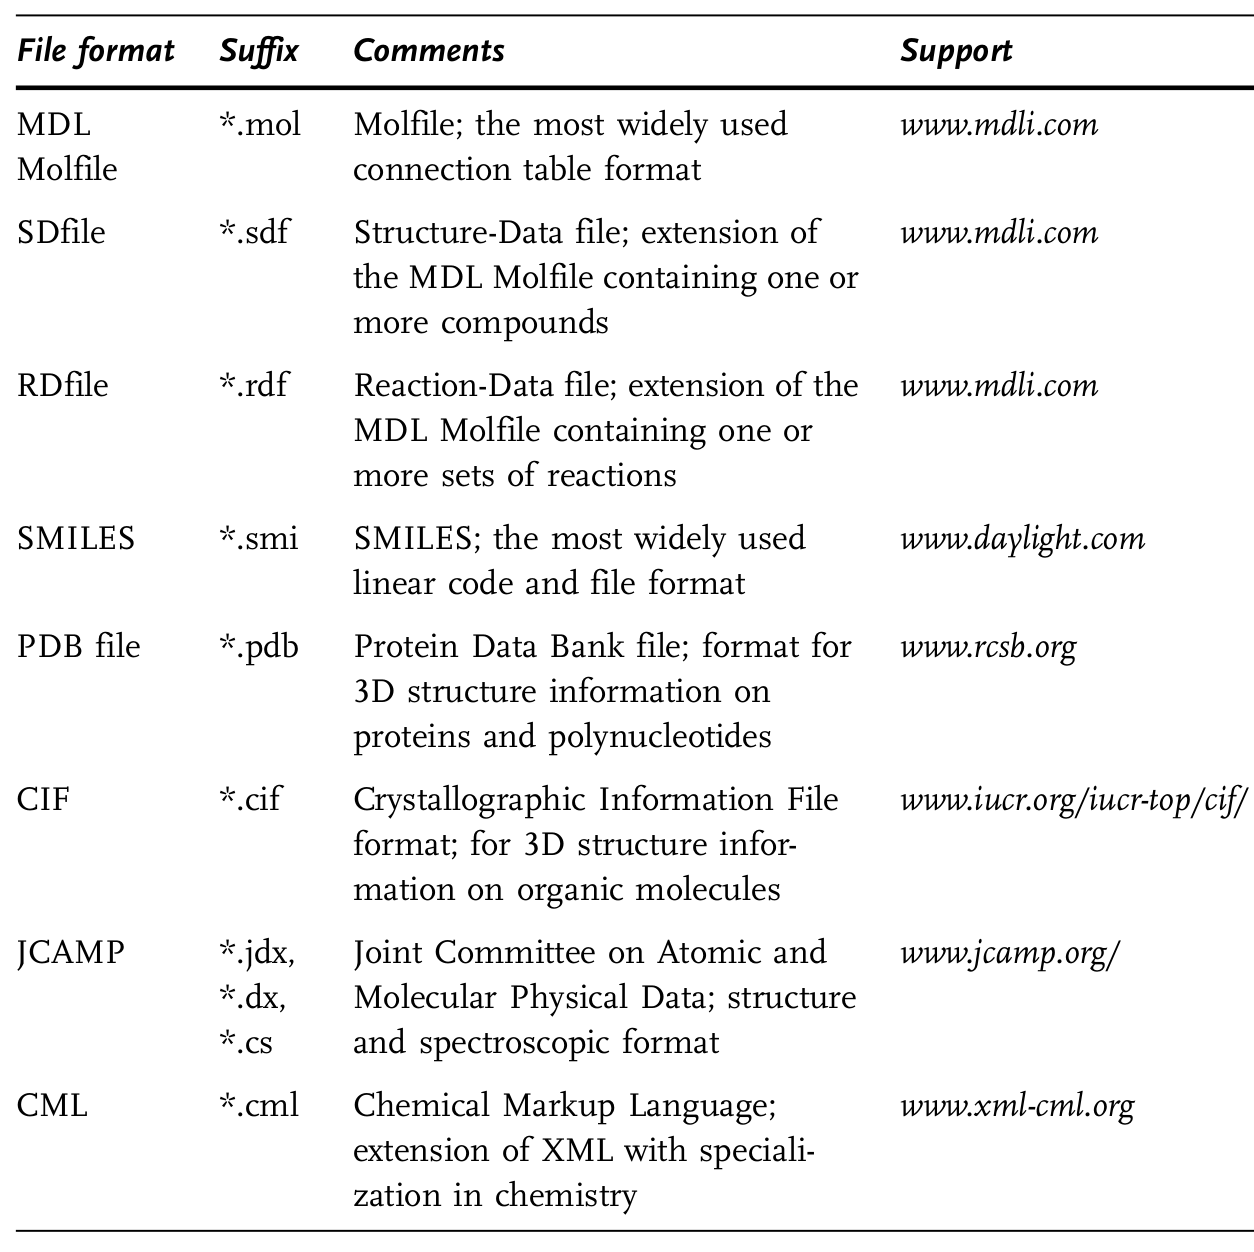
\includegraphics[width=0.5 \linewidth]{images/formats.png}}
\caption{The most important file formats for exchange of chemical information \cite{gasteiger2006chemoinformatics}.}
\end{figure}
\end{frame}

\subsubsection{Molfile}
\begin{frame}
\frametitle{An example of Molfile}
\begin{figure}[h!]
\center{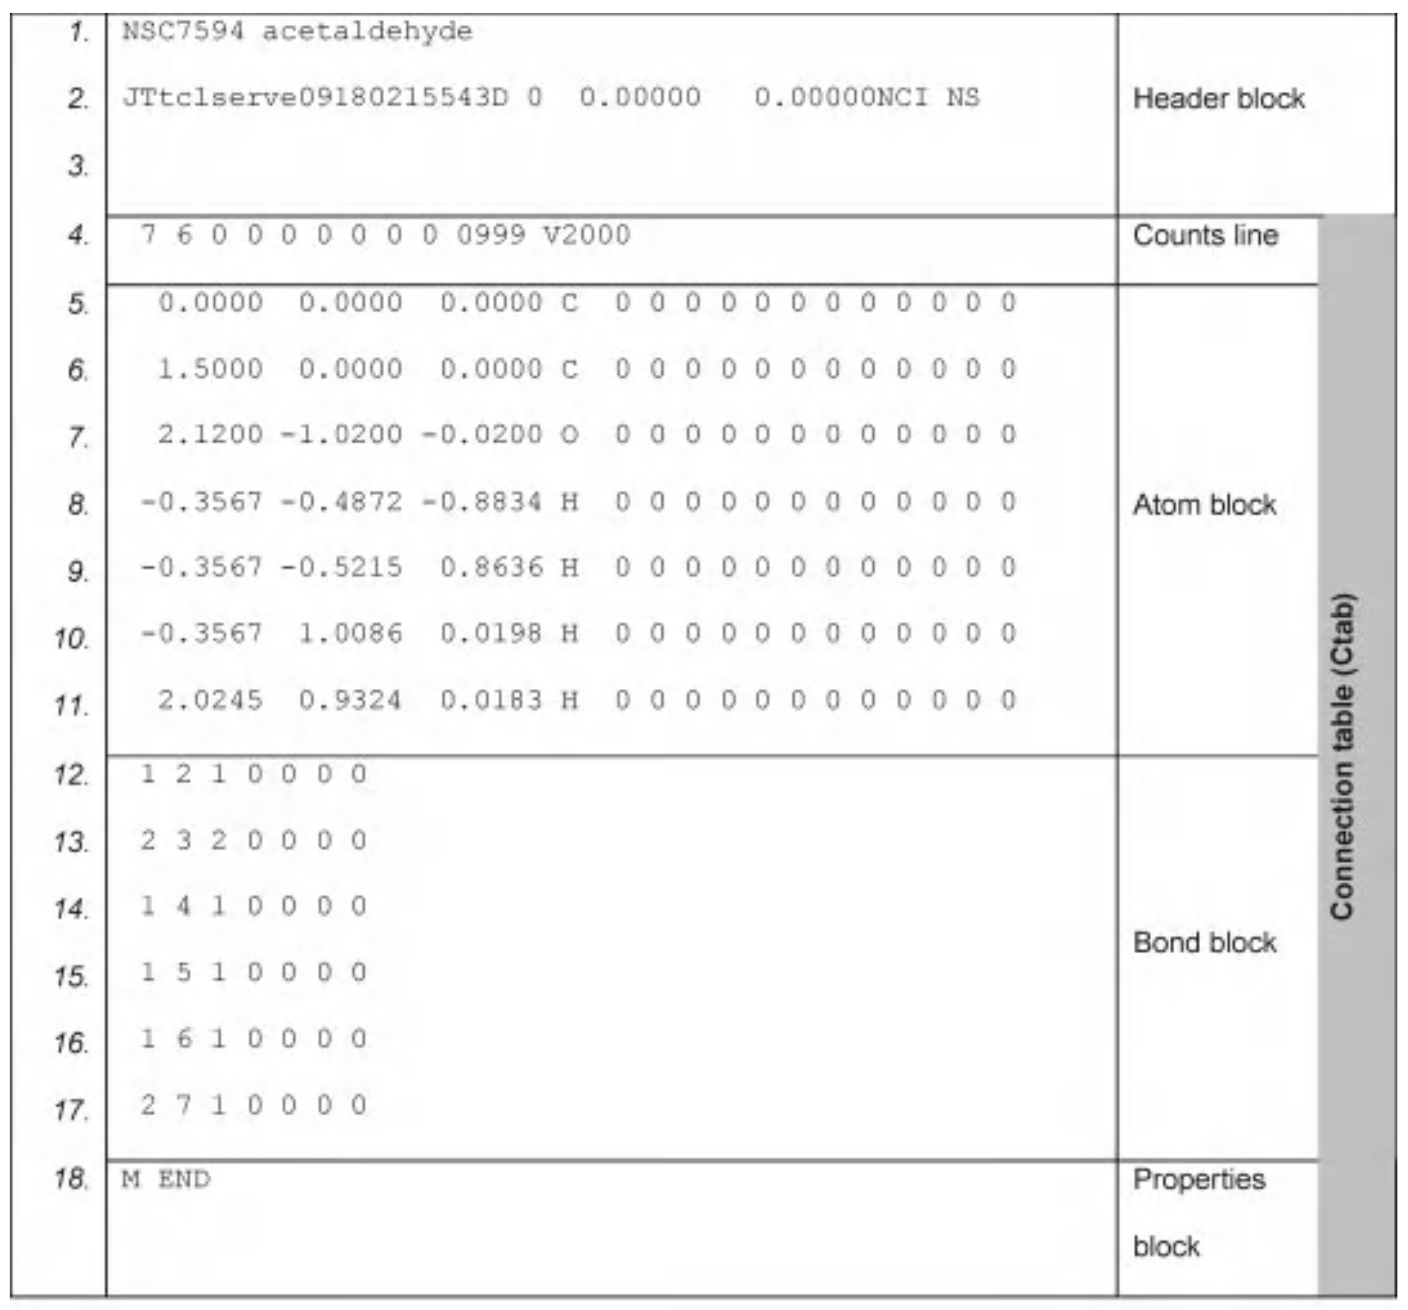
\includegraphics[width=0.6 \linewidth]{images/Molfile.png}}
\caption{Molfile representing the ethanal structure \cite{gasteiger2006chemoinformatics}.}
\end{figure}
\end{frame}

\subsubsection{SDF format}
\begin{frame}
\frametitle{An example of SDF-file}
\begin{figure}[h!]
\center{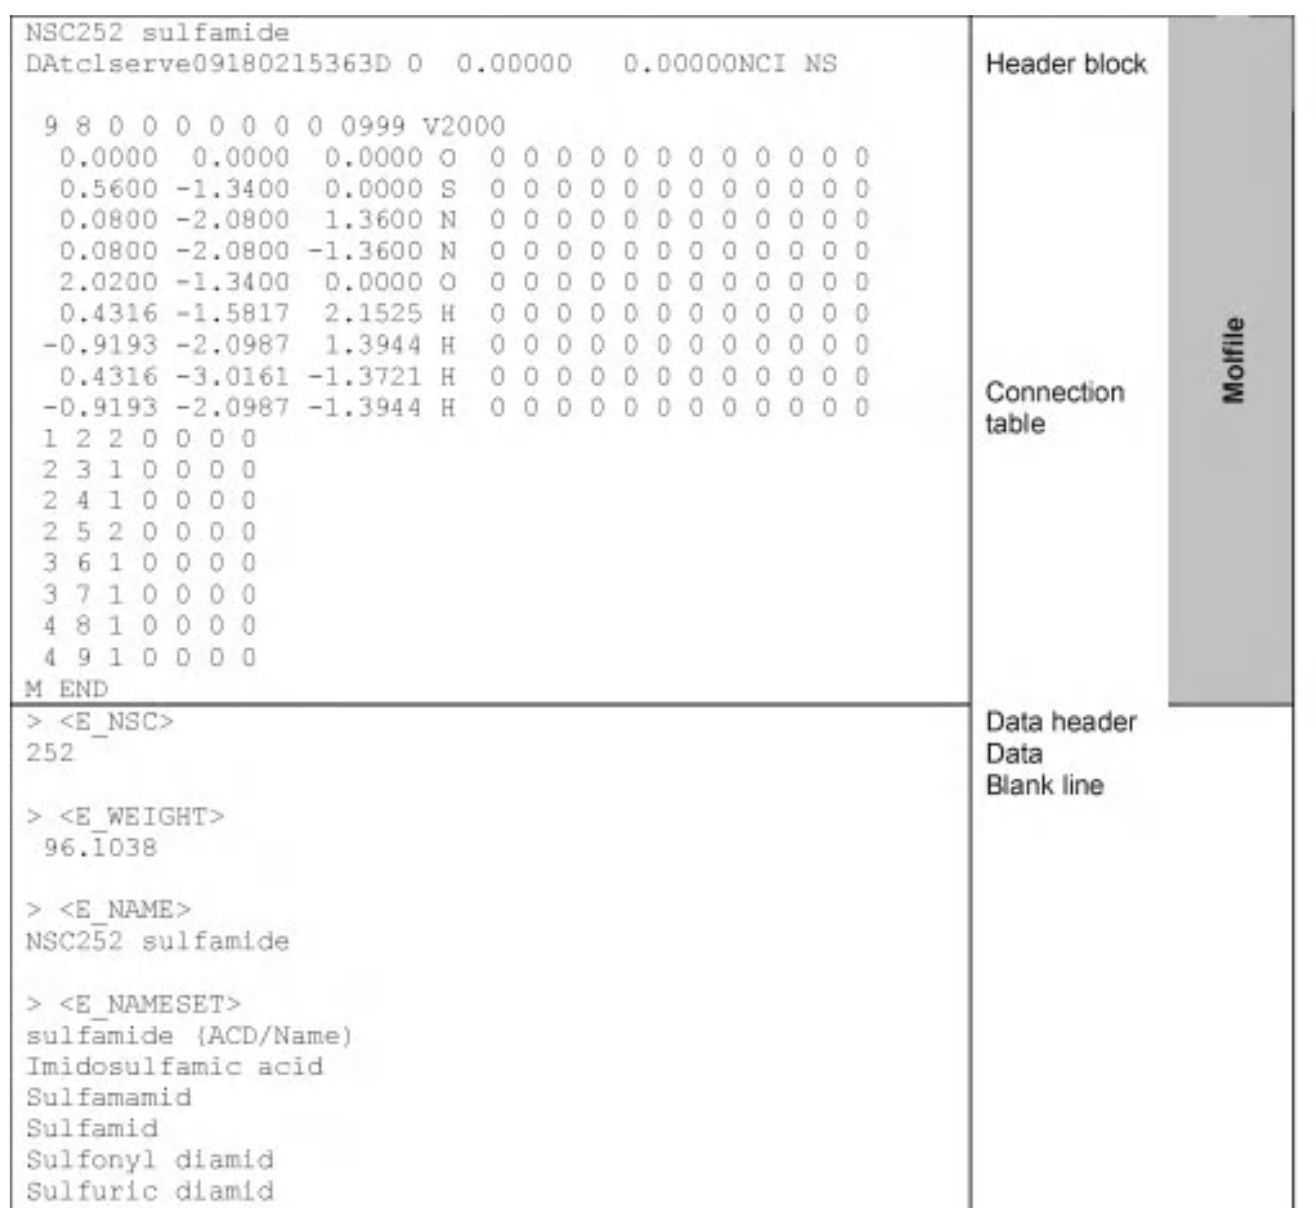
\includegraphics[width=0.6 \linewidth]{images/SDF-file.png}}
\caption{SDF-file representing the ethanal {figure} \cite{gasteiger2006chemoinformatics}.}
\end{figure}
\end{frame}
\section{Canonicalization}
\begin{frame}
\frametitle{Canonicalization}
A structure with n atoms can be numbered in n! different manners and thus has up to n! A process of converting input representation to canonical form is called “canonicalisation” or “canonisation”. Morgan’s algorithm is commonly used for this purpose. It is based on extended connectivity (EC) - considering the degree of neighbours of an atom. The next slide illustrates the principle.
\end{frame}

\subsubsection{Morgan Algorithm}
\begin{frame}
\frametitle{Morgan's algorithm}

\begin{figure}[h!]
\center{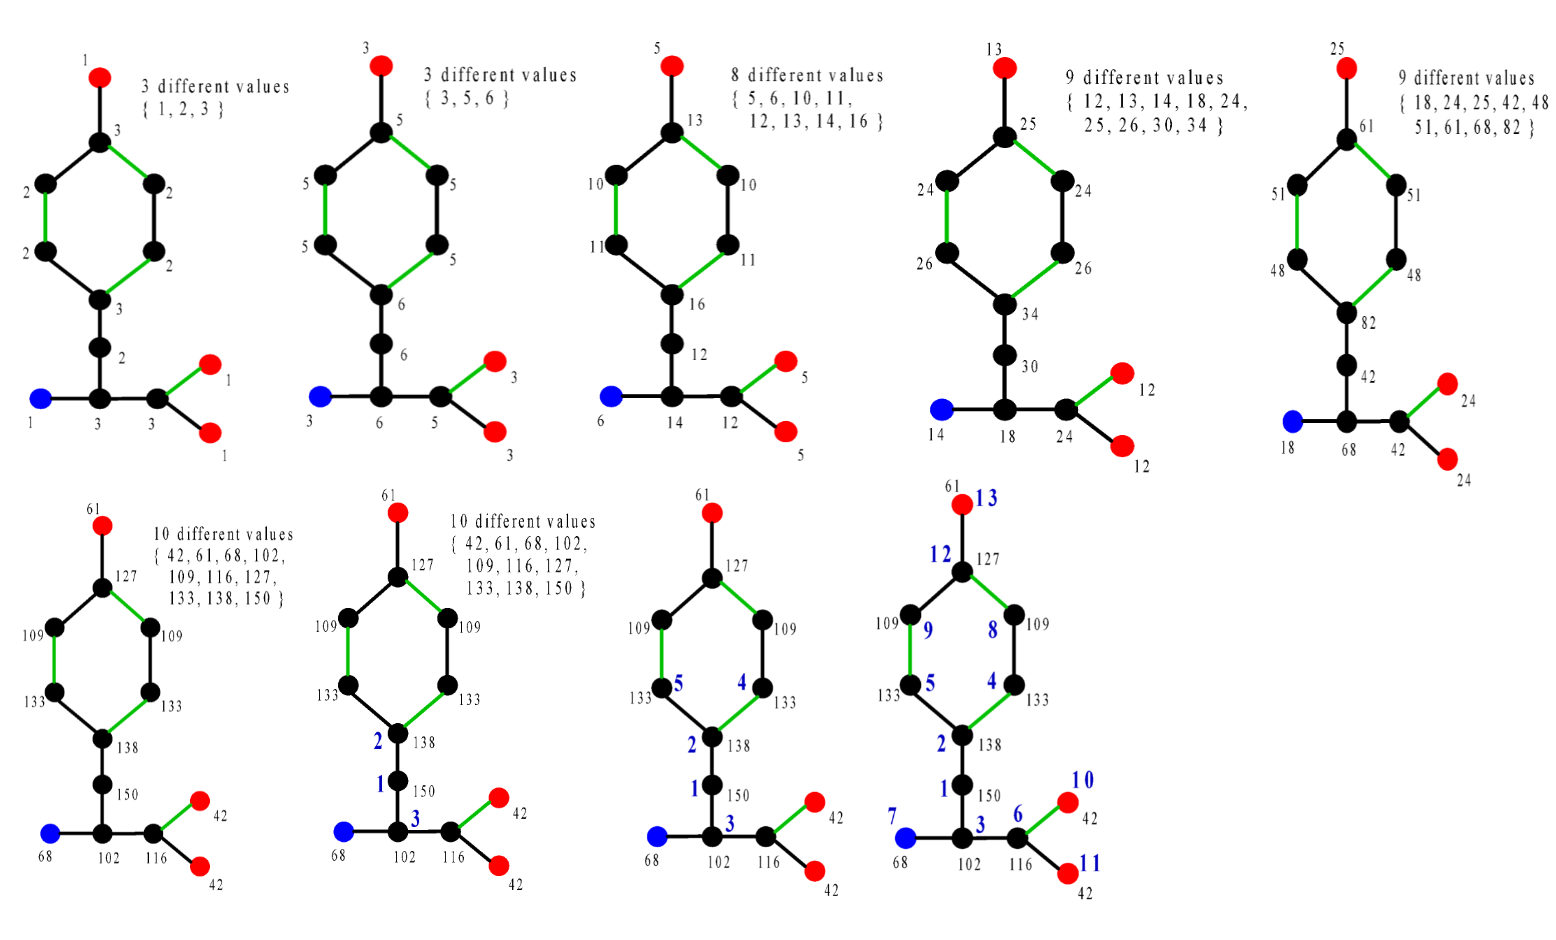
\includegraphics[width=0.9 \linewidth]{images/Morgan_example.png}}
\caption{The Morgan's algorithm}
\end{figure}
\end{frame}

\section{Special Notations of Chemical Structures}
\subsection{Markush Structures}
\begin{frame}
\frametitle{Markush Structures}
Markush structures are mainly used in patents, for protecting compounds related to an invention. The Markush structure diagram is a specific type of representation of a series of chemical compounds. This diagram can describe not only a specific molecule but also various compound families, which is why it is also called a generic structure diagram.
\begin{figure}[h!]
\center{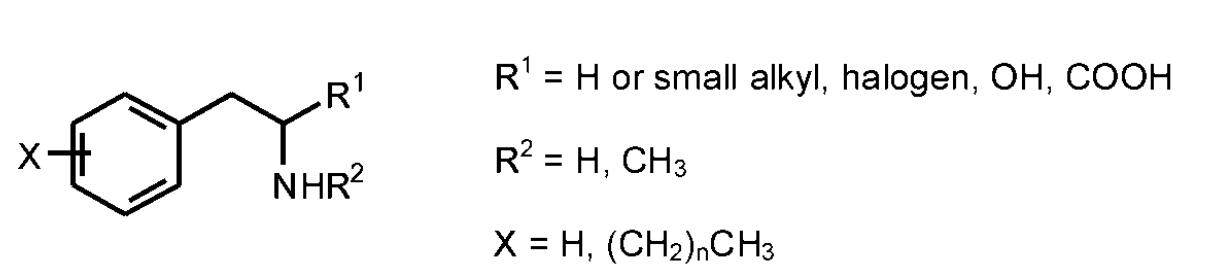
\includegraphics[width=0.9 \linewidth]{images/Markush.png}}
\caption{An example of a Markush Structure \cite{gasteiger2006chemoinformatics}}
\end{figure}
\end{frame}

%------------------------------------------------
\subsection{Fragment Coding}
\begin{frame}
\frametitle{Fragment Coding}
Fragment codes have always played an important role in chemical information systems. Basically, they are indexing expressions of chemical structures. Usually, these are small assemblies of atoms, functional groups, ring systems, etc., which can be specified beforehand. 
\begin{figure}[h!]
\center{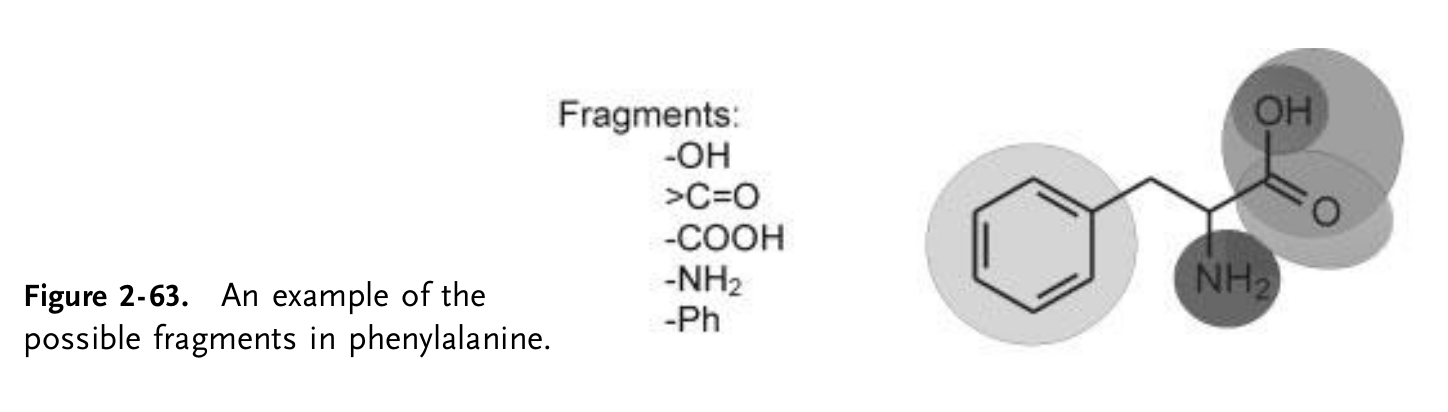
\includegraphics[width=0.9 \linewidth]{images/fragments.png}}
\caption{An example of the possible fragments in phenylalanine \cite{gasteiger2006chemoinformatics}}
\end{figure}
\end{frame}

%------------------------------------------------
\subsection{Fingerprints}
\begin{frame}
\frametitle{Fingerprints}
A fingerprint is a characteristic property used to describe molecules. So a molecule, for example, can be described by the structure or structural keys. These keys indicate whether or not a specific substructure or fragment exists in the molecule. The fragments of chemical structures can be coded in binary keys.
\begin{figure}[h!]
\center{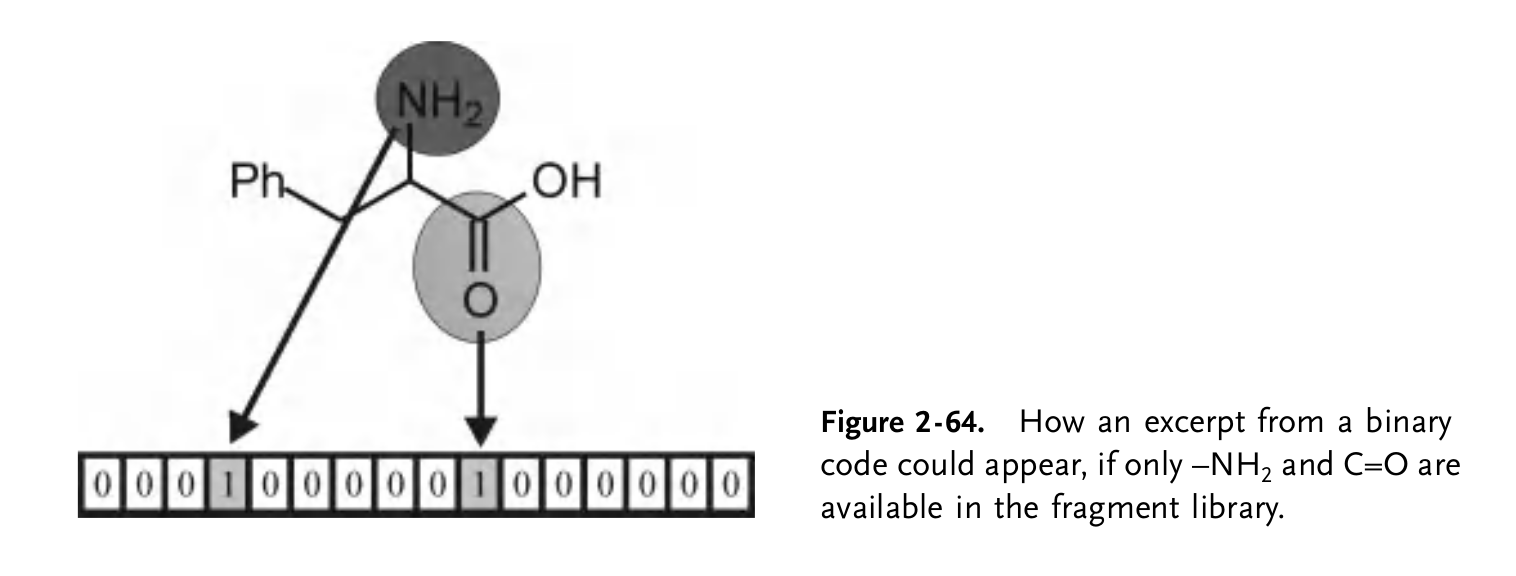
\includegraphics[width=0.9 \linewidth]{images/Fingerprints.png}}
\caption{An example of fingerprints coding \cite{gasteiger2006chemoinformatics}}
\end{figure}
\end{frame}


%------------------------------------------------

\subsection{Hash table & Hashed Fingerprints}
\begin{frame}
\frametitle{Hash table}
A hash table (hash map) is a data structure that implements an associative array abstract data type, a structure that can map keys to values. A hash table uses a hash function to compute an index, also called a hash code, into an array of buckets or slots, from which the desired value can be found. During lookup, the key is hashed and the resulting hash indicates where the corresponding value is stored. 

\begin{figure}[h!]
\center{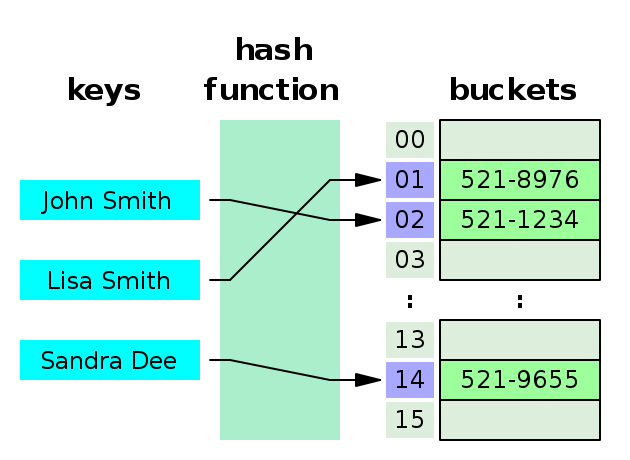
\includegraphics[width=0.4 \linewidth]{images/Hash_table_3_1_1_0_1_0_0_SP.svg.png}}
\caption{Hashing, from \href{https://en.wikipedia.org/wiki/Hash_table}{Wikipedia} \cite{gasteiger2006chemoinformatics}}
\end{figure}
\end{frame}


\begin{frame}
\frametitle{Hashed Fingerprints}
In this procedure, all bonds in the molecule are traversed, starting at an atom and proceeding through several (e.g., seven) bond lengths. Thereby, one receives information about the substructures of the molecule and also about its internal relationships.
\begin{figure}[h!]
\center{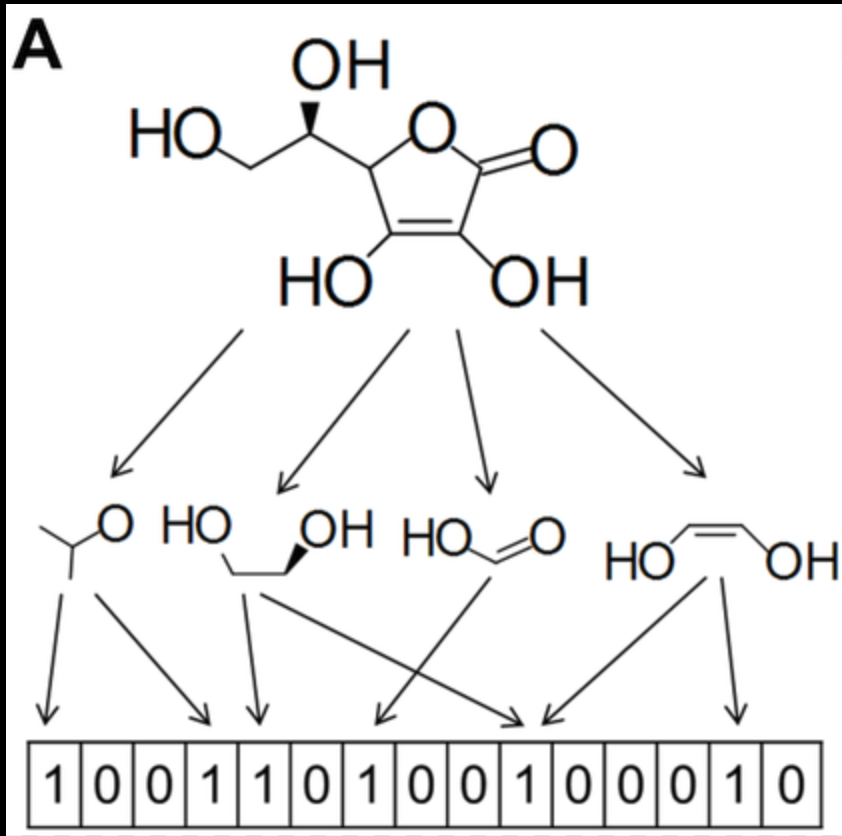
\includegraphics[width=0.4 \linewidth]{images/hashed_fingerprint.png}}
\caption{Hashed Fingerprints \cite{smieja2016average}}
\end{figure}
\end{frame}

\section{References}
\begin{frame}
\frametitle{References}
\printbibliography[heading=none]
\end{frame}


\begin{frame}
\frametitle{TO DO}
\begin{itemize}
    \item Install RDKit
    \item Go through the RDKit's tutorial, commit a notebook with your code to GitHub.
    \item Read chapter 2 (Representation of Chemical Compounds, 15-157 pp) from \cite{gasteiger2006chemoinformatics}
\end{itemize}
\end{frame}
%----------------------------------------------------------------------------------------

\end{document}